\documentclass{report}
\usepackage{titling} % For subtitle
\usepackage{tocloft} % For customizing TOC formatting
\usepackage{soul} % For highlighting text
\usepackage{xcolor}
\usepackage{graphicx}
\usepackage{tabularx} % for automatic column width adjustment


% Manually setting the margins
% \setlength{\textwidth}{\dimexpr 15.4cm}  % Width of text area
\setlength{\textheight}{\dimexpr 23.4cm} % Height of text area
% \setlength{\oddsidemargin}{0.05in}      % Left margin (negative value reduces margin)
% \setlength{\evensidemargin}{0.5in}     % Even page left margin (for two-sided printing)
\setlength{\topmargin}{-0.5in}           % Top margin
\setlength{\headheight}{14pt}            % Space for header (optional)
\setlength{\headsep}{25pt}               % Space between header and text
\setlength{\footskip}{30pt}              % Distance from bottom of text to footer

% Set the main font to Helvetica
\usepackage[scaled]{helvet}
\renewcommand{\rmdefault}{phv}

% Set highlight colour
\sethlcolor{yellow}

\begin{document}

% Title Page Formatting
\begin{figure}
    \centering
    
\includegraphics[width=0.5\textwidth]{Figures/tud_logo.png}
\end{figure}
\title{MSc in Computing - Team Project}
%\title{User Evaluation Report - Magpie (Group 3)}
\author{Anais Blenet\\Saul Burgess\\Yuanshuo Du\\Jessica Fornetti\\Andreas Kraus\\Kaustubh Trivedi}
\date{\today}

% Customizing TOC formatting
\renewcommand{\cfttoctitlefont}{\hfill\Huge\bfseries} % Center TOC title
\renewcommand{\cftaftertoctitle}{\hfill}

\maketitle % Generates the title page

% Table of Contents
\tableofcontents
\newpage

% Main Body
\chapter{Introduction}
\section{Proposed Hypothesis}
Our project's goal is to provide a easy-to-use Geographical Information Service
in Dublin City. In our preliminary research, we couldn’t find a singular
system that allowed users to gain a general overview of public amenities, for
example, parking, bike infrastructure, or public transport. In Ireland and the
United Kingdom, the prevalence of proper digitised records in county
administrations varies wildly (Lynn et al., 2023). Some make use of
state-of-the-art geographical information systems (GIS) while others rely on
spreadsheets which are manually kept up to date. (McGuirk and MacLaran, 2001) A
system that would allow users to quickly inspect a combined dataset grounded in
automatically generated, real-world data could accelerate processes like planning permissions, urban development, or resource allocation.
Prior to user evaluation, exploratory work was conducted in the forms of a
market research survey to answer key demographic \& product questions:
\begin{enumerate}
    \item Who is our primary target user?
    \item What kind of amenity data do they access and how?
    \item What devices/tools do they primarily use?
    \item Are they satisfied with those tools?
    \item Would they consider Magpie useful in filling the gaps in their
          toolset?
\end{enumerate}
Responses from the survey further allowed us to confirm our target demographic
(figure 1.1), find out the proportion of users using amenity data for their work
(figure 1.2), what type of amenity data  they require access to (figure 1.3) and
why current tools are unsatisfactory (figure 1.4).
\begin{figure}
    \centering
    \begin{minipage}{0.45\textwidth}
        \centering
        \fbox{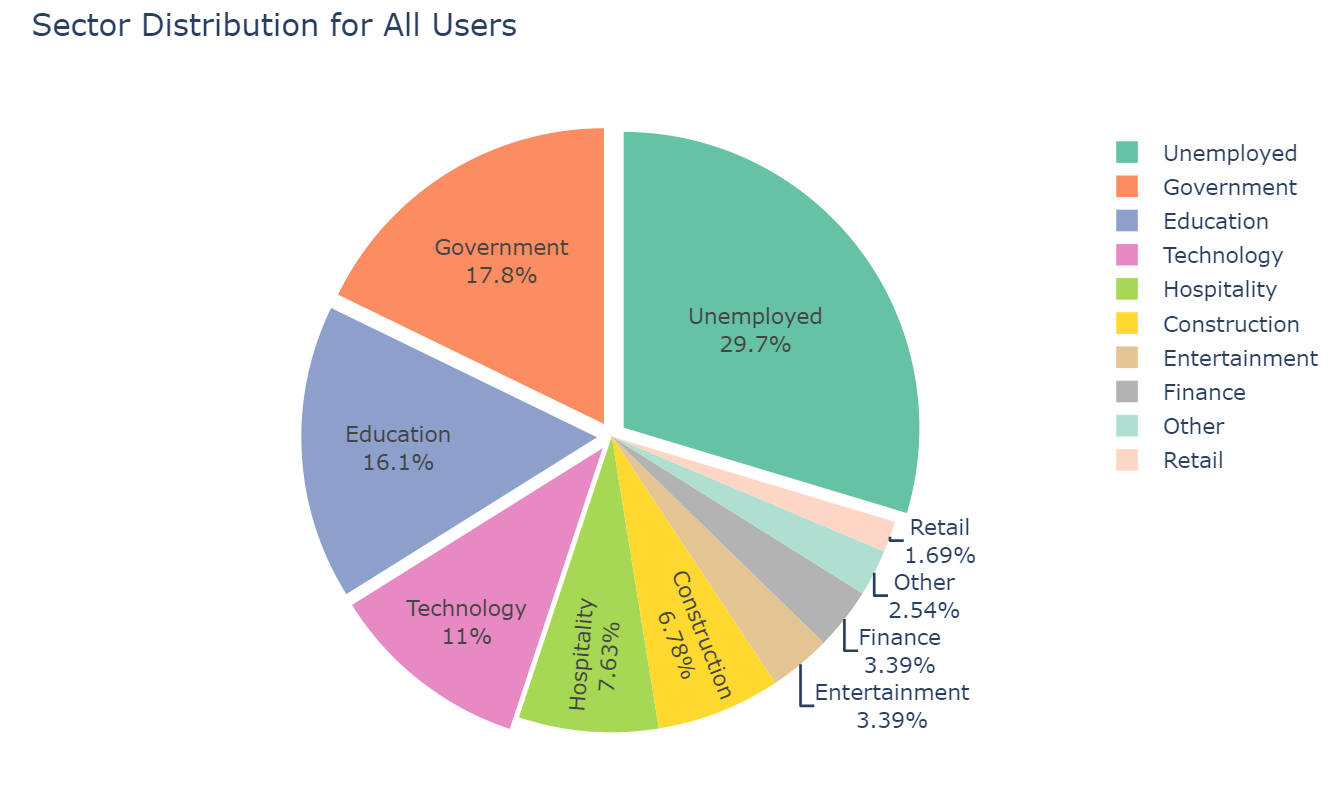
\includegraphics[width=\textwidth]{Figures/fig1.png}}
        \caption{Target user sectors}
        \label{fig:plot1}
    \end{minipage}
    \hfill
    \begin{minipage}{0.45\textwidth}
        \centering
        \fbox{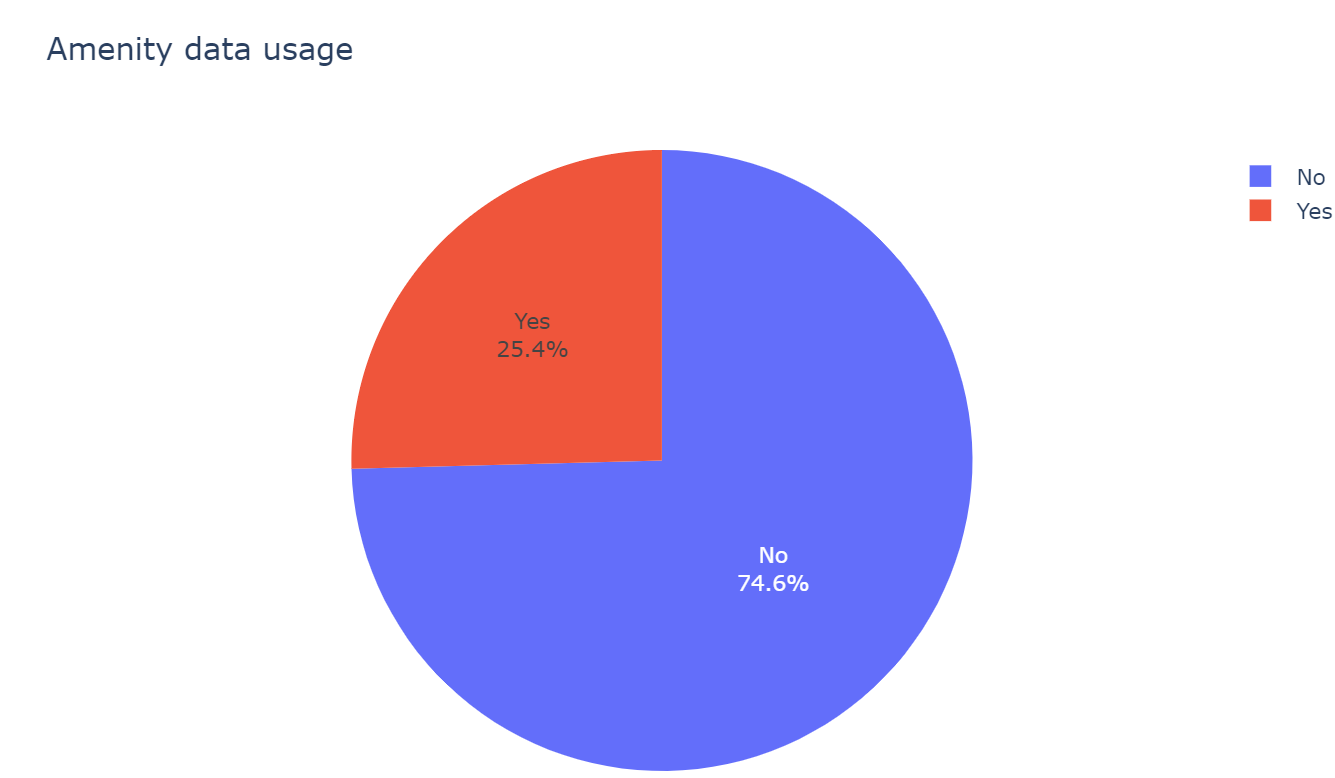
\includegraphics[width=\textwidth]{Figures/fig2.png}}
        \caption{Amenity Access distribution}
        \label{fig:plot2}
    \end{minipage}
\end{figure}
These responses also cemented the need of Magpie (figure 1.5) for both casual
users (User A) \& professionals who require amenity data (User B).
\begin{figure}
    \centering
    \begin{minipage}{0.5\textwidth}
        \centering
        \fbox{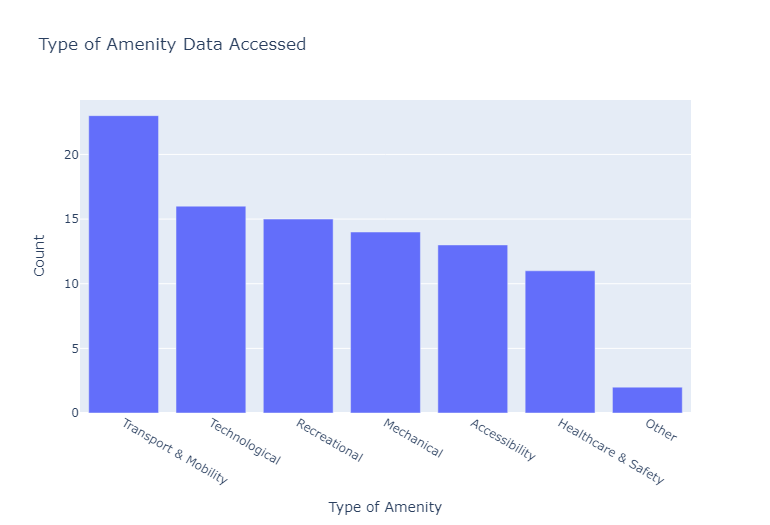
\includegraphics[width=\textwidth]{Figures/fig3.png}}
        \caption{Current amenity data accessed}
        \label{fig:plot3}
    \end{minipage}
    \hfill
    \begin{minipage}{0.6\textwidth}
        \centering
        \fbox{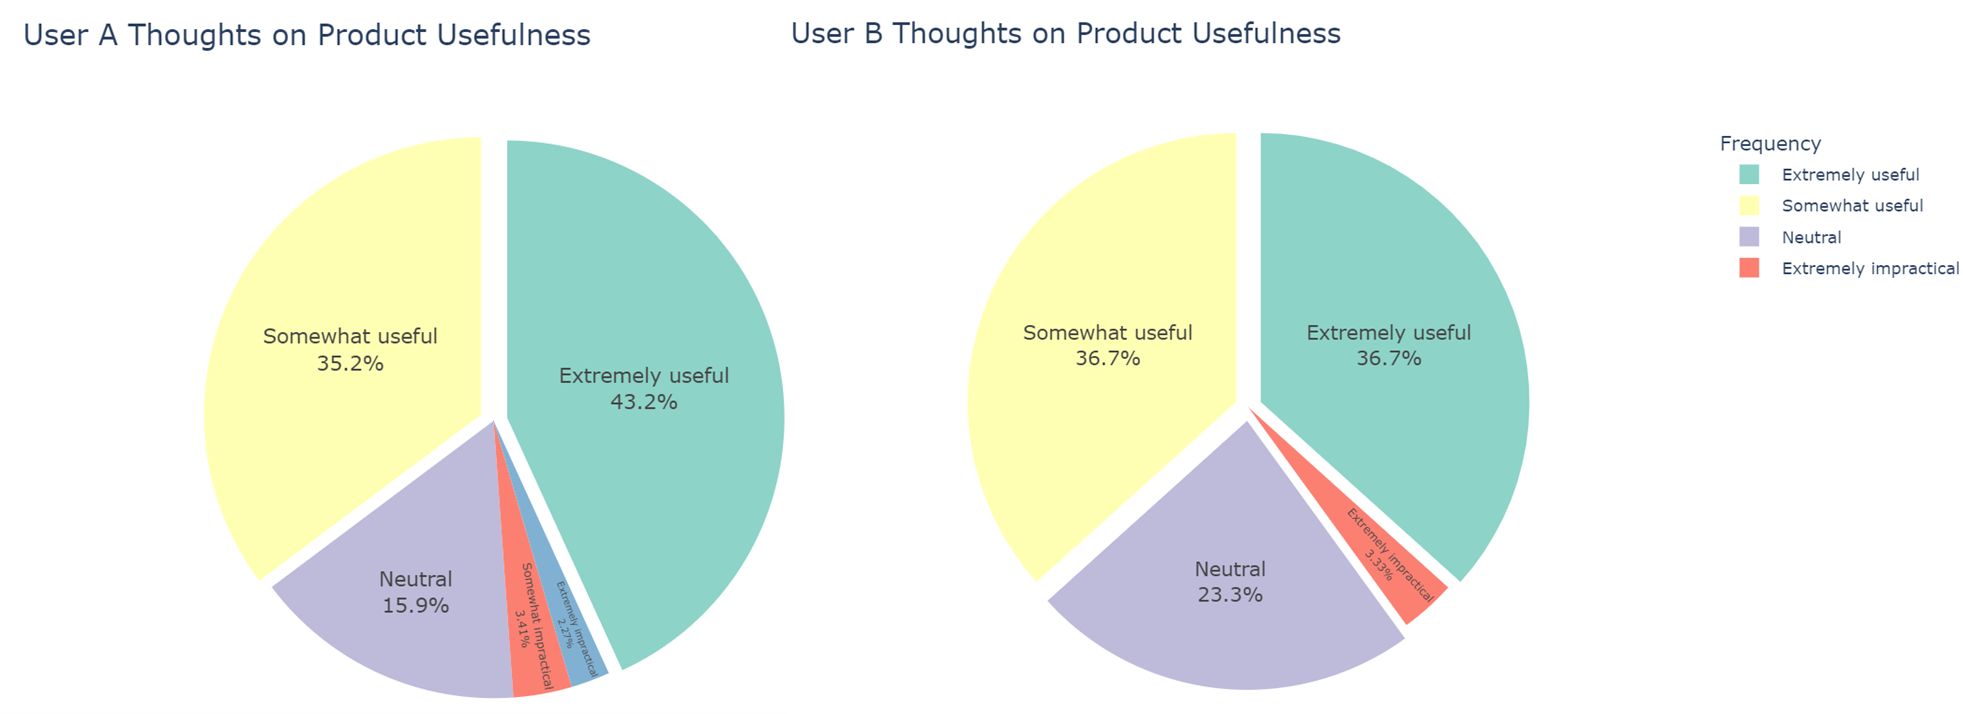
\includegraphics[width=\textwidth]{Figures/fig4.png}}
        \caption{Current tools \& satisfaction rate}
        \label{fig:plot4}
    \end{minipage}
    \hfill
    \begin{minipage}{0.6\textwidth}
        \centering
        \fbox{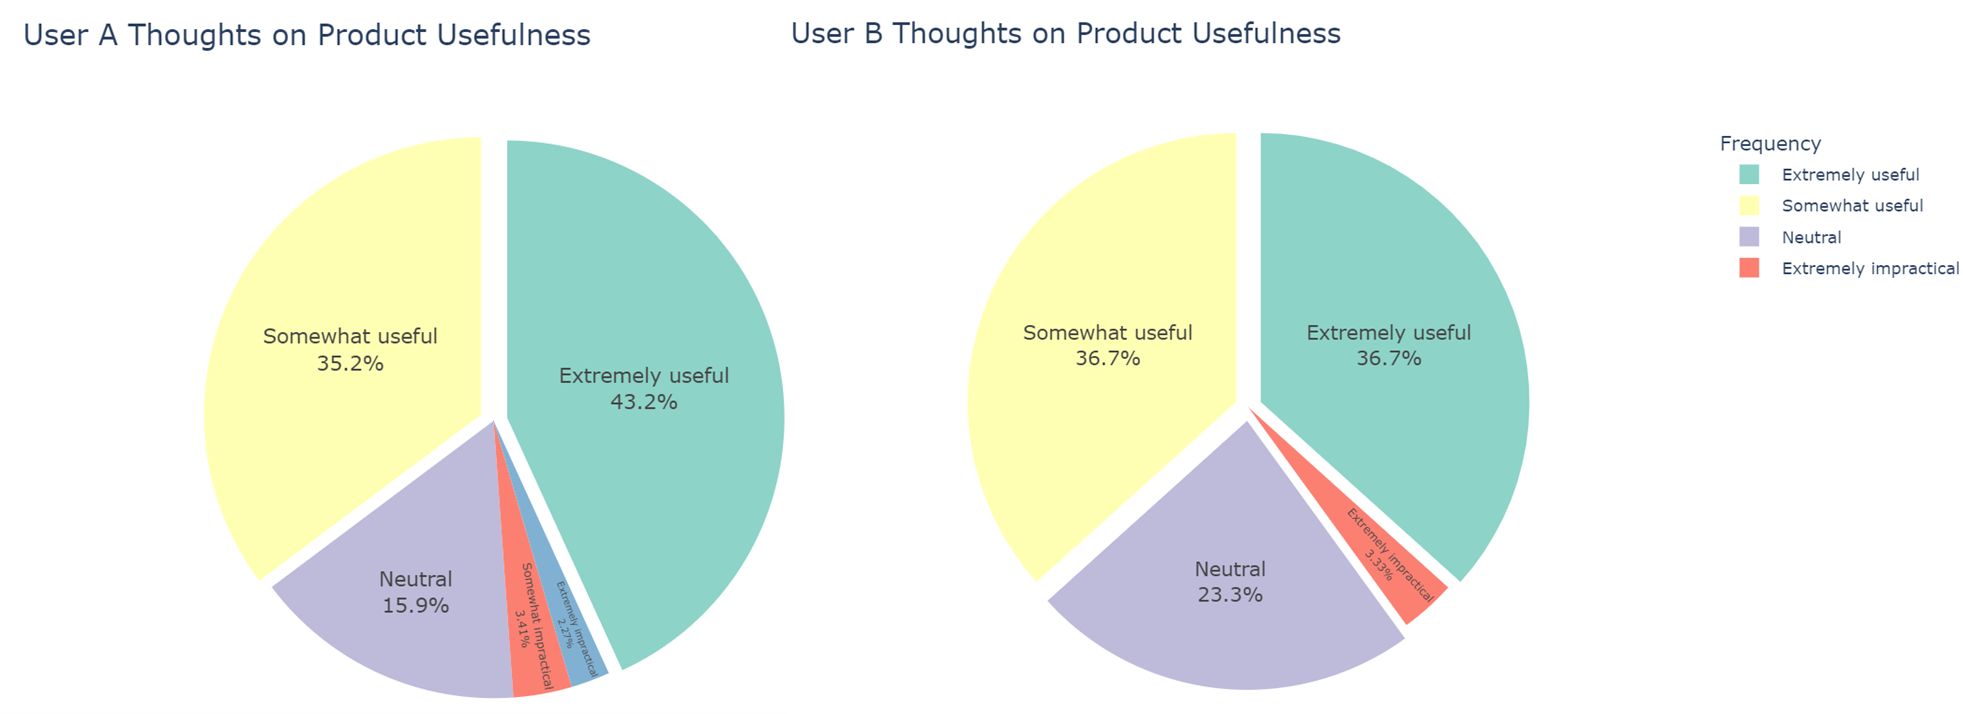
\includegraphics[width=\textwidth]{Figures/fig5.png}}
        \caption{Magpie potential}
        \label{fig:plot5}
    \end{minipage}
\end{figure}

\noindent{}The survey also helped us implement additional features (figure
1.6,1.7 \& 1.8) prior to the user evaluation such as a dashboard with search functionality and filters.\\ \\

\begin{figure}
    \centering
    \begin{minipage}{0.45\textwidth}
        \centering
        \fbox{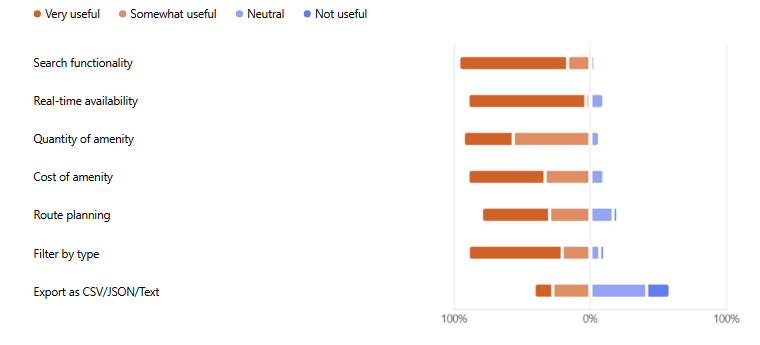
\includegraphics[width=\textwidth]{Figures/fig6.png}}
        \caption{Additional features rating}
        \label{fig:plot6}
    \end{minipage}
    \hfill
    \begin{minipage}{0.45\textwidth}
        \centering
        \fbox{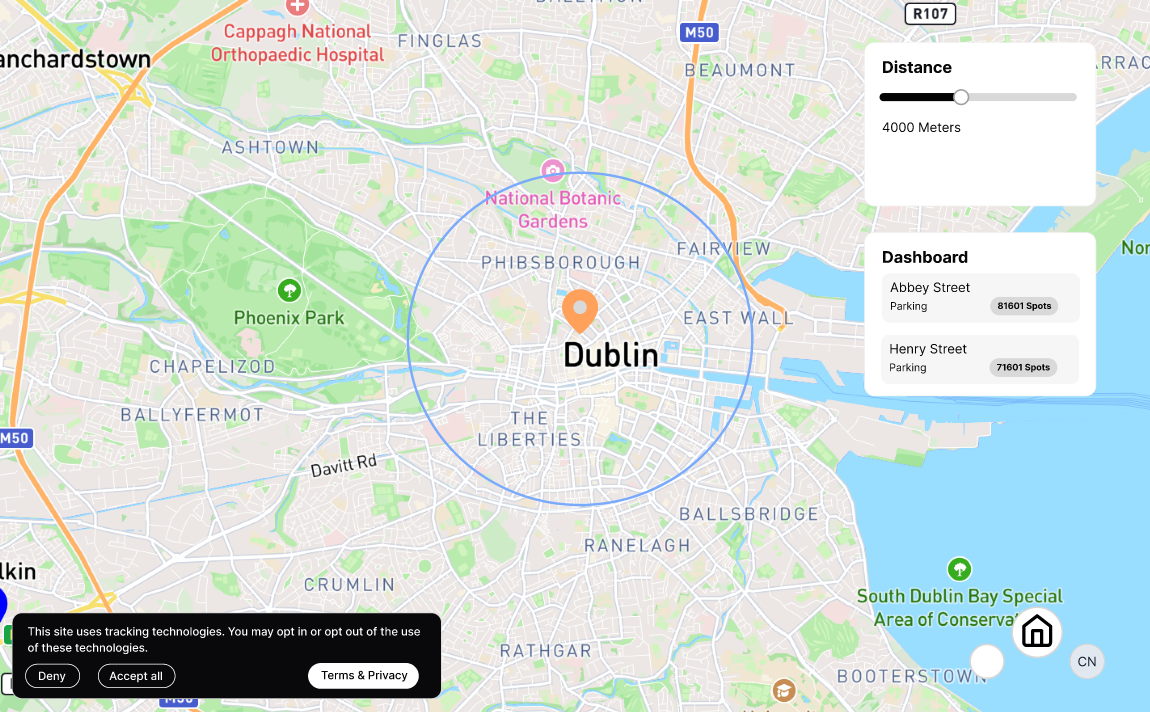
\includegraphics[width=\textwidth]{Figures/fig7.png}}
        \caption{Version 1 of high fidelity prototype}
        \label{fig:plot7}
    \end{minipage}
    \hfill
    \begin{minipage}{0.45\textwidth}
        \centering
        \fbox{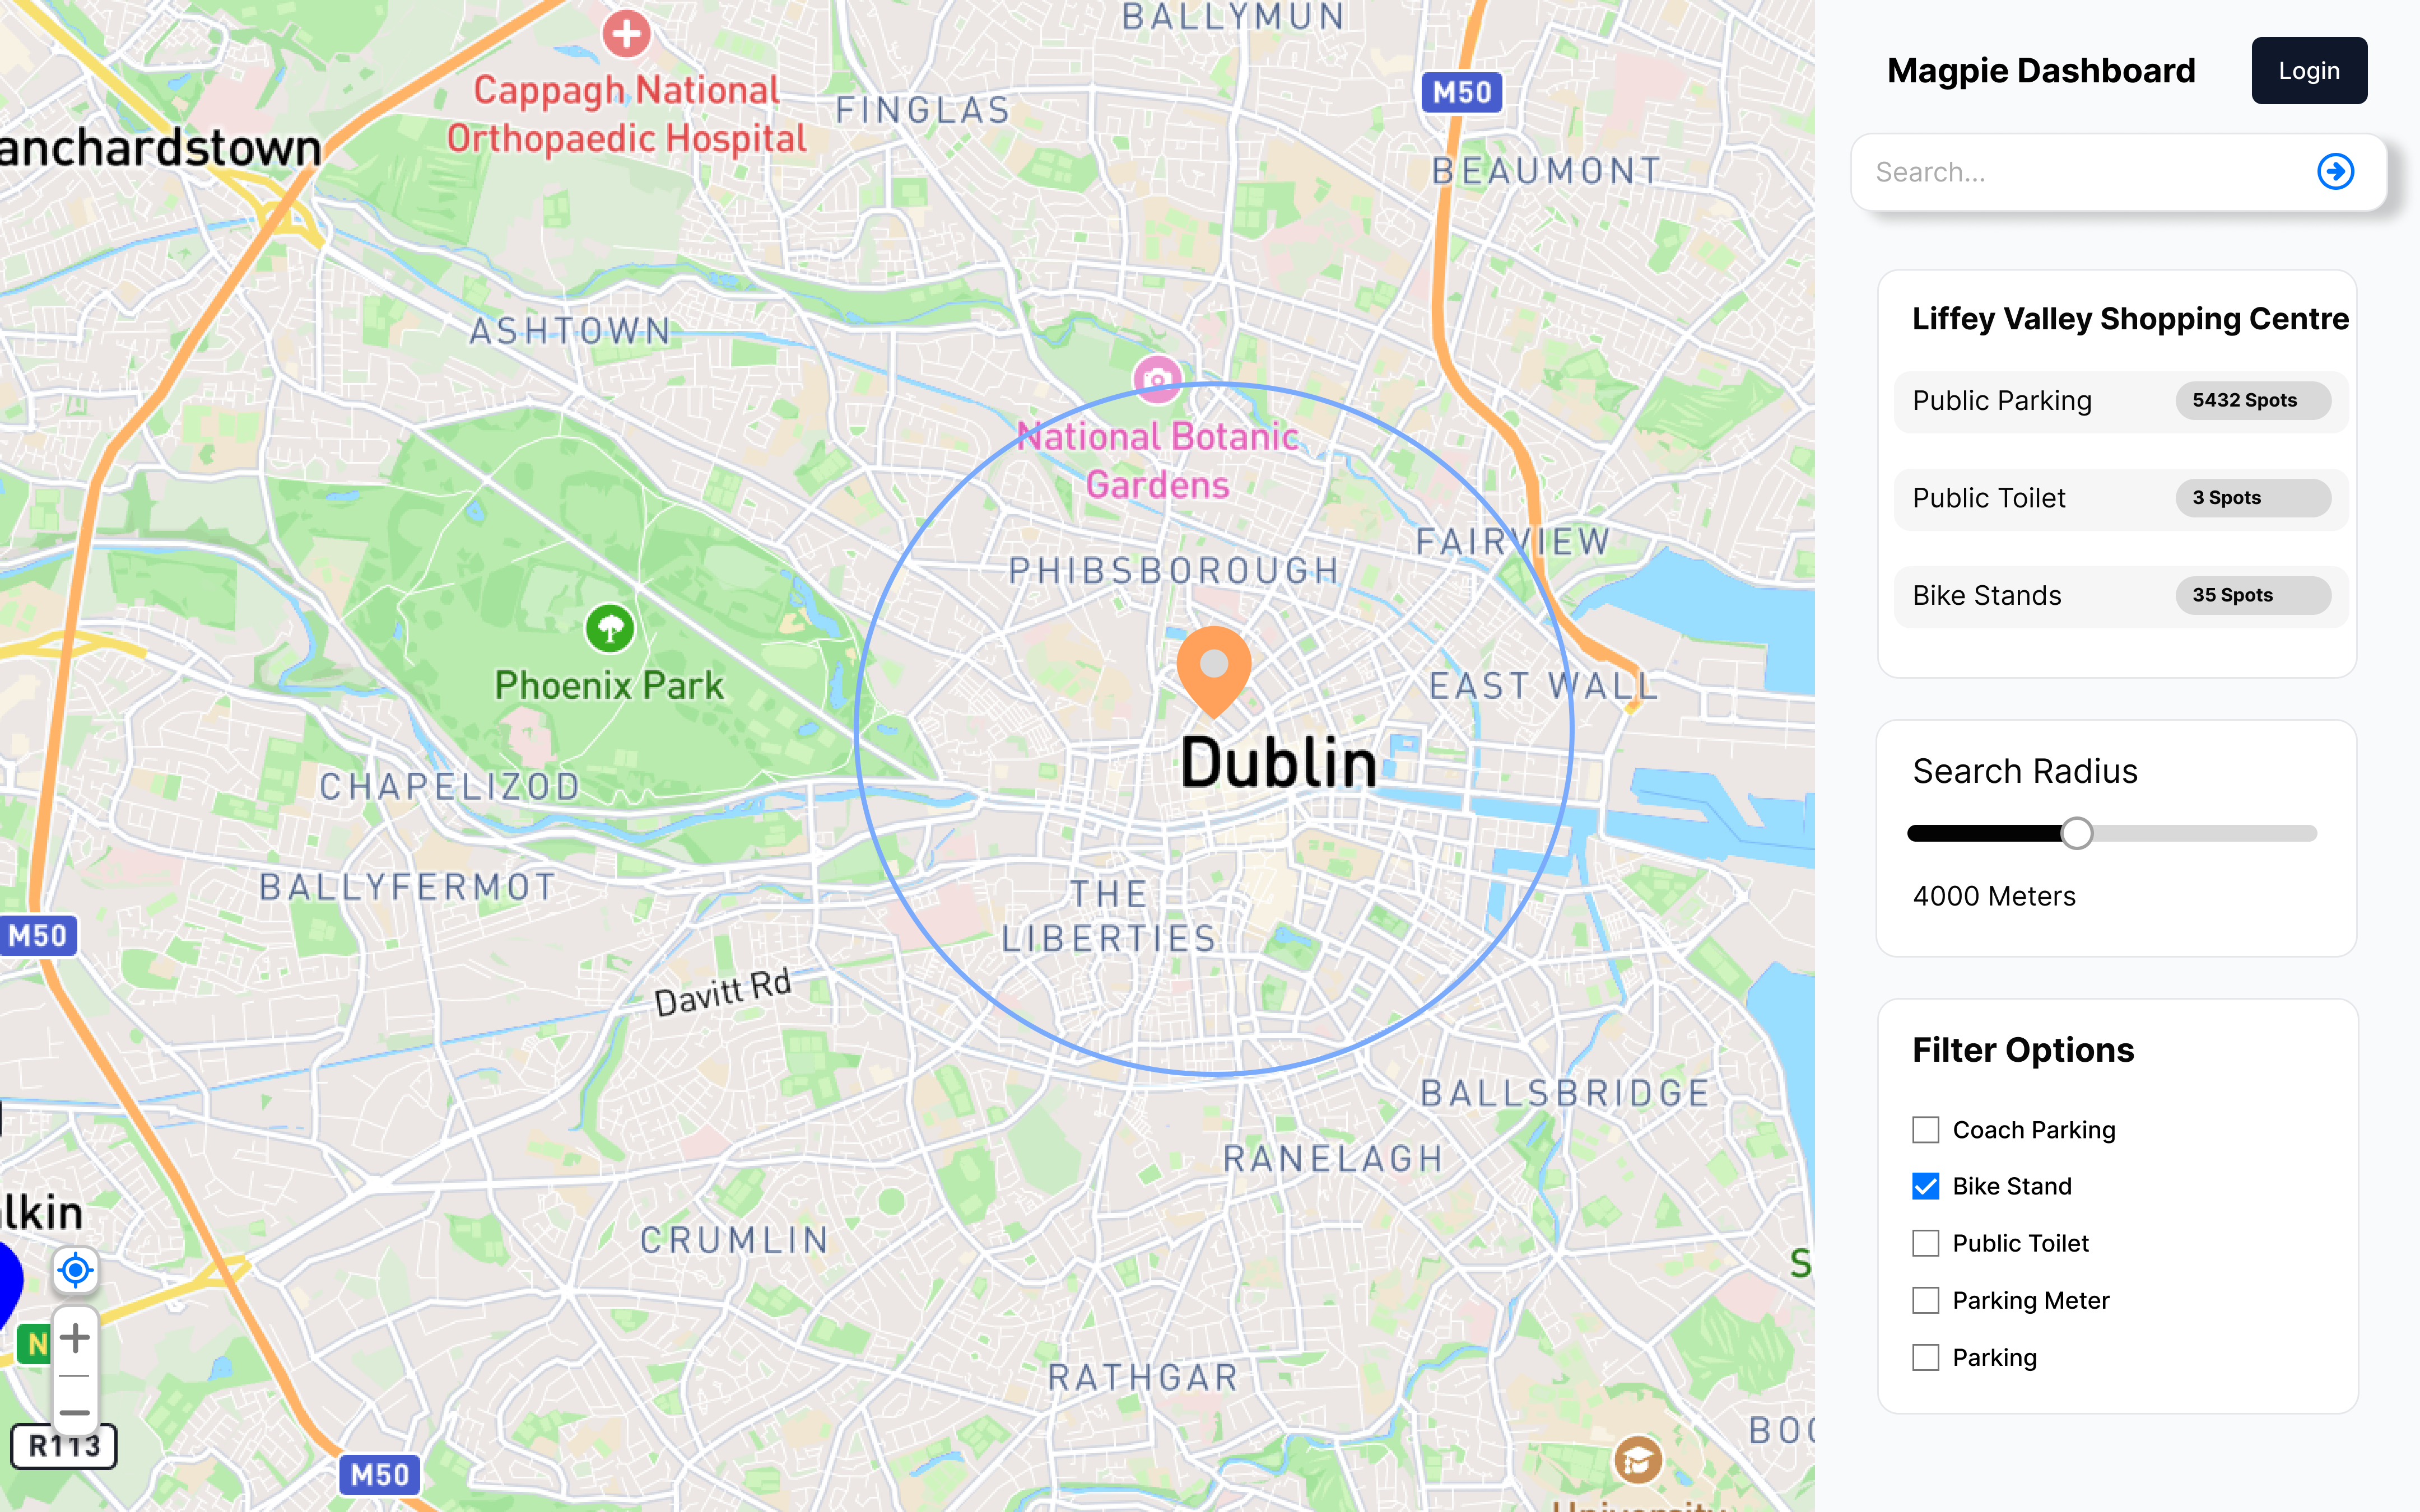
\includegraphics[width=\textwidth]{Figures/fig8.png}}
        \caption{Version 2 of high-fidelity prototype}
        \label{fig:plot8}
    \end{minipage}
\end{figure}

\noindent{}Magpie has remedied the first challenge of fragmented information on
amenities, and through this user evaluation, we hope to address the second challenge
which is making the access to this information easy, quick \& accessible.

\chapter{Experimental Methods}
The goal of the user evaluation is to gain feedback from real users, learn if
Magpie works as expected and assess how user-friendly it is. We will be using 2
main methods to collect both qualitative data through open-ended questions, and
quantitative data from multiple choice questions from which we will derive
insights to improve the Magpie user experience.
\section{Usability Testing}
\subsection{Casual Think-Aloud Protocol}
\begin{enumerate}
    \item \underline{Objective:} Obtain quick feedback on frontend features during the development \& implementation process
    \item \underline{Conditions:} Oral feedback, written notes
    \item \underline{Methodology:}
          \begin{enumerate}
              \item Request feedback from users in the immediate circle
              \item Work together with the user through the app and the feature we want to test
              \item Observe workflow of the user, discuss freely on their manner of interaction with the feature
              \item Build on this feedback to make changes or implement the new feature
          \end{enumerate}
    \item \underline{Baseline \& Evaluation metrics:} No baseline; user experience is evaluated "casually", meaning informally \& subjectively at each person's discretion. This method serves as the "Step 0" of usability testing in helping us implement "Draft 1" of new features.
\end{enumerate}
\subsection{Uncontrolled (Remote)}
\begin{enumerate}
    \item \underline{Objective:} Evaluate user experience in an uncontrolled
          environment, assess overall functioning of Magpie \& identify any
          potential usability issues
    \item \underline{Conditions:} Online followed up by survey
    \item \underline{Methodology:}
          \begin{enumerate}
              \item Share the link to Magpie online to wide user-base to request their participation in testing Magpie
              \item Send them survey to rate their experience
              \item Analyse the responses \& present the results
          \end{enumerate}
    \item \underline{Baseline \& Evaluation metrics:} No baseline; user experience will be evaluated through a 10 question satisfaction survey (figure 2.1) to collect quantitative data only. Minimum number of responses is 20 to produce valuable insights.
\end{enumerate}

\begin{figure}
    \begin{minipage}{\textwidth}
        \centering
        \fbox{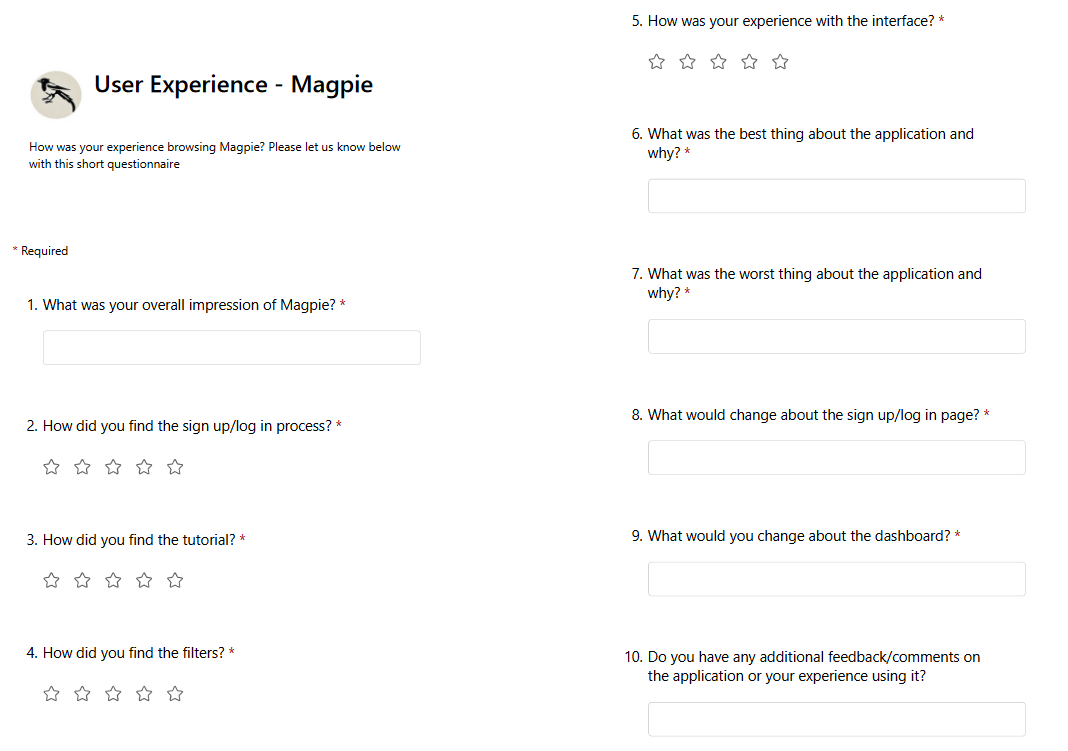
\includegraphics[width=\textwidth]{Figures/fig9.png}}
        \caption{User Experience survey}
        \label{fig:plot9}
    \end{minipage}
\end{figure}

\subsection{Controlled (Remote)}
\begin{enumerate}
    \item \underline{Objective:} Analyze how users interact with Magpie in a
          controlled environment guided by specific instructions and tasks to complete
          \& identify any potential usability issues
    \item \underline{Conditions:} Online through videoconference tools
          (Zoom/GoogleMeet/Teams)
    \item \underline{Methodology:}
          \begin{enumerate}
              \item Reach out to casual users who left their contact email in the market research survey \& request their participation
              \item Schedule the test session
              \item Conduct the test session
              \item Collect qualitative data from users through open-ended questions pre-during-post test
              \item Collect quantitative data from users through user experience survey post-test
              \item Analyse responses \& present results
          \end{enumerate}
    \item \underline{Baseline \& Evaluation metrics:} User experience will be evaluated through a range of metrics shown below:
          \begin{enumerate}
              \item Task Success Rate
              \item Time on Task
              \item Difficulty of Task
              \item Errors
          \end{enumerate}
          These will measure how the users are working through a series of pre-defined tasks (Table 2.1). These are the most common usability metrics and they tend to have moderate correlation with each other to suggest an overlap (Sauro et.al 2009).  Averaging them together allows us to generate a Single Usability Metric (SUM) which summarizes the user experience running through those tasks. These metrics will be measured by filling score cards and through observation \& discussion with the users. In addition, quantitative data will be collected through a user experience survey shown in figure 2.1.
\end{enumerate}
\begin{table}[htbp]
    \centering
    \begin{tabular}{|p{5cm}|p{2.5cm}|p{2cm}|p{2cm}|p{3.5cm}|}
        \hline
        \textbf{Task}                    & \textbf{Expected Completion}      & \textbf{Target Time} & \textbf{Difficulty (1-5)} & \textbf{Typical Errors}                     \\
        \hline
        Load Magpie application          & User sees login page              & 5s                   & 1                         & Network timeout, browser compatibility      \\
        \hline
        Access Terms and Privacy         & User views policy page            & 10s                  & 1                         & None expected                               \\
        \hline
        Return to login                  & User returns to main login        & 5s                   & 1                         & Navigation confusion                        \\
        \hline
        Sign up new account              & Complete registration             & 2m                   & 2                         & Invalid email format, password requirements \\
        \hline
        Complete onboarding              & Finish all tutorial steps         & 3m                   & 2                         & Skipping steps, confusion about progression \\
        \hline
        Place cursor and set 250m radius & Radius circle visible at location & 30s                  & 3                         & Incorrect radius size, wrong location       \\
        \hline
        Zoom to road name level          & Street names visible              & 20s                  & 2                         & Over/under zooming                          \\
        \hline
        Zoom out to full radius          & Complete circle visible           & 15s                  & 2                         & Losing circle location                      \\
        \hline
        New location with 400m radius    & Larger radius at new spot         & 30s                  & 3                         & Radius adjustment issues                    \\
        \hline
        Select parking meter filter      & Parking meters visible            & 15s                  & 2                         & Filter selection confusion                  \\
        \hline
        Remove parking meter filter      & Filter removed                    & 10s                  & 1                         & Filter deselection issues                   \\
        \hline
        Add toilets and WiFi filters     & Both amenities shown              & 20s                  & 2                         & Multiple filter confusion                   \\
        \hline
        New location with 100m radius    & Smaller radius at new location    & 25s                  & 3                         & Precise radius adjustment                   \\
        \hline
        %Export as PNG                    & Image downloaded                  & 15s                  & 1                         & Download location confusion                 \\
        %\hline
        Exit onboarding at step 3        & Tutorial closed                   & 10s                  & 1                         & Exit button not found                       \\
        \hline
        Logout                           & Return to login page              & 10s                  & 1                         & Menu navigation issues                      \\
        \hline
    \end{tabular}
    \caption{Magpie User Testing Protocol}
    \label{tab:user-testing-protocol}
\end{table}
\subsection{Field-test (Remote)}
\begin{enumerate}
    \item \underline{Objective:} Analyze how users interact with Magpie in a
          controlled environment guided by their own tasks for their day-to-day work
          \& identify any potential usability issues
    \item \underline{Conditions:} Online through videoconference tools
          (Zoom/GoogleMeet/Teams)
    \item \underline{Methodology:}
          \begin{enumerate}
              \item Reach out to professional users who left their contact
                    email in the market research survey \& request their participation
              \item Schedule the test session
              \item Conduct the test session
              \item Collect qualitative data from users through open-ended questions pre-during-post test
              \item Collect quantitative data through user experience survey post-test
              \item Analyse responses \& present results
          \end{enumerate}
    \item \underline{Baseline \& Evaluation metrics:} No baseline; user
          experience will be evaluated on their feedback through the user experience survey in figure 2.1, complemented by observational analysis.
\end{enumerate}
\section{Expert Review}
We requested an expert review from UI/UX professional Andrea Curley. The goal of this review is to evaluate the user interface of Magpie, rate its user-friendliness in regards to UI/UX general guidelines and the application's compliance with the EAA (European Accessibility Act).\\
The expert review will be conducted online through a videoconference meeting on Teams and will take the following form:
\begin{enumerate}
    \item Presentation of Magpie
    \item Free-roaming of the application by Professor Curley
    \item Questionnaire
    \item Discussion \& end of review
\end{enumerate}
The questionnaire includes questions on visual design, information architecture, data quality \& integration, technical performance, compliance and overall assessment of Magpie as shown in Table 2.3.
\begin{table}[h!]
    \centering
    \caption{Expert Review Questionnaire}
    \label{tab:table3}
    \begin{tabularx}{\textwidth}{|p{0.6\textwidth}|X|X|}
        \hline
        \textbf{Question}                                                                                                                                                                                                                & \textbf{Question type} & \textbf{Answer type} \\ \hline
        How user friendly is the log-in/sign up page?                                                                                                                                                                                    & Closed                 & Multiple choice      \\ \hline
        How user-friendly is the on-boarding process                                                                                                                                                                                     & Closed                 & Multiple choice      \\ \hline
        How effective is the visual hierarchy of the information on the dashboard?                                                                                                                                                       & Closed                 & Multiple choice      \\ \hline
        Rate the clarity of the map visualization                                                                                                                                                                                        & Closed                 & Multiple choice      \\ \hline
        How intuitive is the organization of amenity data categories?                                                                                                                                                                    & Closed                 & Multiple choice      \\ \hline
        Rate the following features from Worst (1) to Best (5) = Onboarding, Radius scaling, filter options completeness, profile menu                                                                                                   & Closed                 & Scale                \\ \hline
        How comprehensive is the amenity data coverage for Dublin city?                                                                                                                                                                  & Closed                 & Multiple choice      \\ \hline
        How valuable do you think this tool would be for the following use cases - 1: Not valuable at all, 5: Extremely valuable = Urban planning, Resource allocation, Planning permissions, Event planning, Education, Travel planning & Closed                 & Scale                \\ \hline
        Any additional comments on why this tool would useful/impractical for the above use cases?                                                                                                                                       & Open-ended             & Text                 \\ \hline
        Evaluate the following technical aspects from Worst (1) to Best (5) = Loading speed, System responsiveness, Data update frequency, Filter functionality, Radius selection                                                        & Closed                 & Scale                \\ \hline
        Rate the application's compliance with the items below from Worst (1) to Best (5) = Accessibility, GIS data standards, GDPR                                                                                                      & Closed                 & Scale                \\ \hline
        Any additional comments regarding our application?                                                                                                                                                                               & Open-ended             & Text
    \end{tabularx}
\end{table}

\chapter{Results}
\section{Usability testing}
\subsection{Casual Think-Aloud Protocol}
\subsubsection{Onboarding feature implementation}
Onboarding feature was tested with two users, one casual and the other professional. The professional user had little issues with the onboarding
feature, and found it clear and went through each step smoothly without questions. The casual user attempted to click on the highlighted user
interface elements during the tutorial, which is not possible. They expressed that they would've liked to interact with the highlighted elements.\\
Due to the limitation of the feature, we are not able to make this interaction possible. However, a deeper black was added to the screen overlay to better indicate
that elements are not clickable. Figure 3.1 shows the before and figure 3.2 the after. \\
\begin{figure}
    \centering
    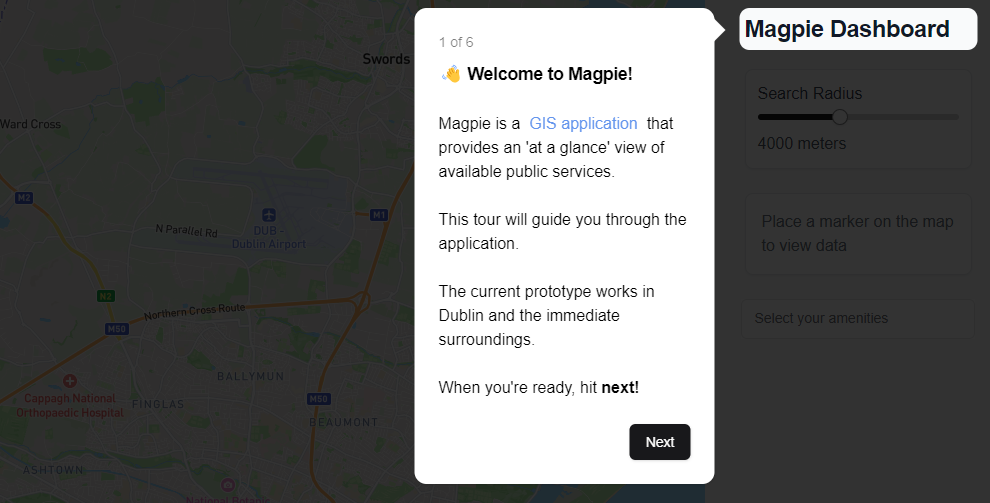
\includegraphics[width=0.5\textwidth]{Figures/fig10.png}
    \caption{Onboarding before overlay change}
    \label{fig:plot10}
    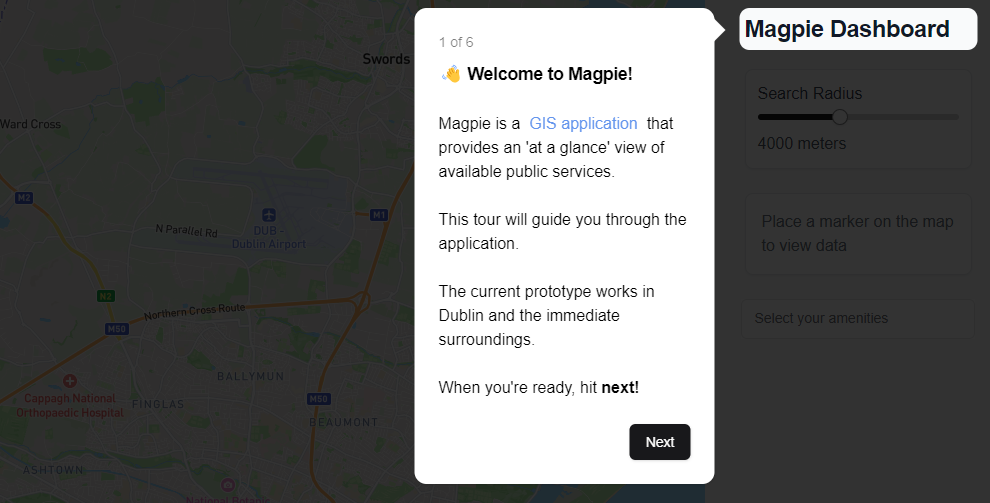
\includegraphics[width=0.5\textwidth]{Figures/fig11.png}
    \caption{Onboarding after overlay change}
    \label{fig:plot11}
\end{figure}
In addition, Gifs were also added to the onboarding elements to indicate what each
button does. The onboarding feature was tested again with the same users and
they both found it more intuitive

\subsubsection{Avatar implementation}
In the early development stage, we collected feedback from roommates and colleagues who pointed out that the avatar should display correctly on different devices and have the function of changing pictures such as uploading or selecting.
At the same time, some people also reported that according to their experience, they may encounter difficulties such as inflexible image cropping and slow upload speed.\\
Based on this feedback, we adjusted the default avatar to make it responsive on different devices and are currently developing the "add/upload profile picture". We will also pay attention to the concerns mentioned throughout the development of the profile feature.
\begin{figure}
    \centering
    \fbox{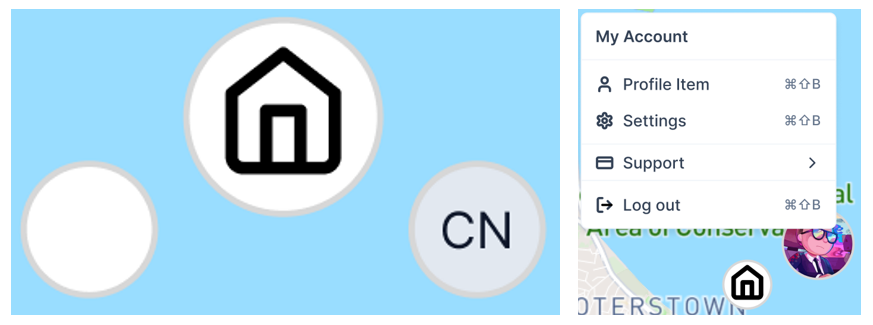
\includegraphics[width=0.5\textwidth]{Figures/fig14.png}}
    \caption{First version of avatar/profile button}
    \label{fig:plot14}
    \fbox{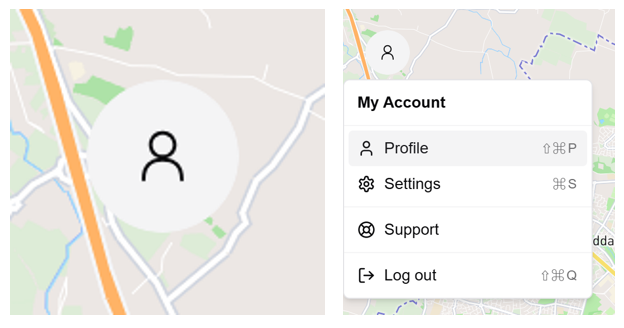
\includegraphics[width=0.5\textwidth]{Figures/fig15.png}}
    \caption{Second version of avatar/profile button}
    \label{fig:plot15}
\end{figure}

\subsubsection{Dashboard Implementation}
5 users were provided unrestricted access to the dashboard and encouraged to interact naturally with the system while providing verbal feedback. This approach allowed us to observe authentic user behavior and identify potential usability issues.\\

\textbf{Map Interface: }
Users quickly figured out how to move around and zoom in and out without needing instructions. However, users less familiar with digital maps mentioned they'd prefer having traditional '+' and '-' buttons for zooming rather than relying on the mouse wheel. Some also found it tricky to keep track of where they were in relation to the wider city area, suggesting that a small overview map in the corner would help them stay oriented. A few users also mentioned that when they selected an area, they weren't always sure if their selection had registered properly, indicating we could make the visual feedback more obvious when an area is selected.\\

\textbf{Radius Control: }
Users found the radius selection tool intuitive to use. When they moved the slider, they appreciated seeing the circle size change immediately on the map, giving them instant feedback about their selection. However, several users mentioned it would be helpful to type in specific radius values when they needed exact measurements. Some also suggested having quick-select buttons for commonly used distances, like 100m, 250m, and 500m, which would save time for frequent searches. A few users noted that the circle outline could be hard to see in certain areas of the map, and recommended making it more visible, perhaps with a bolder or more contrasting color.\\

\textbf{Amenities Filter: }
This part of the dashboard received mixed feedback. Most users found the basic selection and deselection process straightforward, though three users specifically mentioned they initially missed the scrollable nature of the list. Two users suggested grouping similar amenities together, particularly noting how parking-related options (Parking, Parking Meter, Accessible Parking) could be consolidated under one category.\\ All users successfully used the filter, but four out of five mentioned that a search function would be helpful when looking for specific amenities in the list. The most common praise was for the clear 'x' button to remove selections, while the most frequent criticism was the lack of visual hierarchy and categorization in the list. One user specifically noted that larger icons on the map would improve visibility and recognition of different amenity types.\\

\textbf{Map Legend Dashboard: }
All users appreciated the clear display of amenity counts and consistent labeling format (Spots, Locations, etc.), but three  noted confusion about zero values staying visible in the list. Two users specifically mentioned that adding icons to the dashboard would help quick identification, while all users noted the helpful distinction between different unit types (Spots vs. Locations vs. Points). The most significant improvement request was for better visual hierarchy and the ability to collapse categories to reduce scrolling. \\

\subsection{Uncontrolled (Remote)}
In Progress
\subsection{Controlled (Remote)}
In Progress
\subsection{Field-test (Remote)}
In Progress

\section{Expert review}
The review provided very valuable insights on Magpie's workflow, user interface and technical components. These were the main takeaways:\\ \\
\textbf{Landing Page: }
Upon loading Magpie, Professor Curley was directly taken to the mapview, which was not supposed to happen. After the review, we investigated the cause of this event and uncovered a bug in the authentication which we have been working on. Following this event, she suggested creating a landing page or some sort of introduction to ease the user into discovering Magpie.\\ \\
\textbf{Onboarding: }
Due to the bug explained above, the onboarding did not automatically start as it should have upon login. Nevertheless, Professor Curley said that the user may want to intuitively press on the elements being highlighted during the tutorial, as she tried to do. This adds to the feedback received during casual testing for the implementation of this feature. Unfortunately, due to a technical limitations we are not able to solve it, only provide make certain changes to dissuade the user of doing so.\\
In addition, Professor Curley suggested there should be an option to exit the tutorial at any time for users who don't want to sit through it. Lastly, the tutorial shoud be more visually striking and engaging in order to leave a lasting impression on the user.\\ \\
\textbf{Dashboard \& Map: }
Currently, the hierarchy of items on the dashboard does not make sense to the average, and is not intuitive to use. All the amenities are displayed when only one is selected (as shown in figure 3.3) and their count displays zero, which the user might interpret as there are zero other amenities in the area in addition to the one I selected.\\
The icons on the map are not visible enough, and zooming in \& out on the map may not be intuitive to the range of users and devices. Adding zoom buttons could help bridge that gap. \\
Currently, Professor Curley noted that there is a disconnect between the map and the dashboard whereas they should be looked as one. She suggested adding amenity icons to the dashboard to help bridge that gap.\\ \\
\begin{figure}
    \fbox{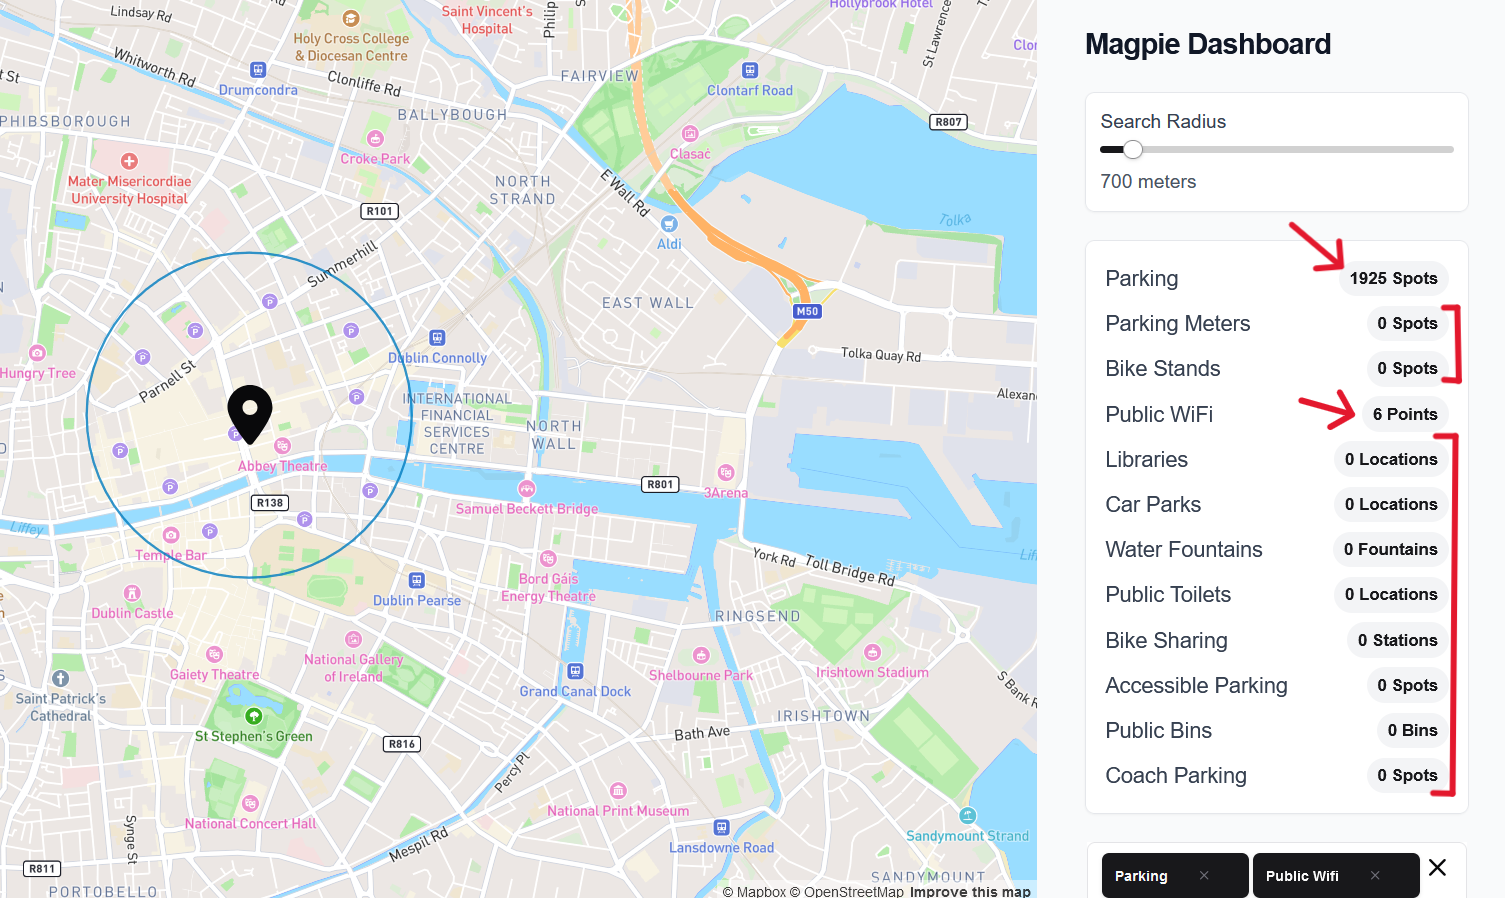
\includegraphics[width=\textwidth]{Figures/fig12.png}}
    \caption{Current dashboard \& map when 2 amenities are selected}
    \label{fig:plot12}
\end{figure}
\textbf{Filters: }
If there are no amenities found in the radius of search, a message should pop up to tell the user so. Currently, it is not very clear if there are amenities present in the chosen area especially due to the small size \& faded color of the icons. \\ \\
\textbf{Log in/sign up: }
When trying to log in with credentials that don't exist, the system should return a proper error such as "username doesn't exist". Log out and account sign up went smoothly. Professor Curley questioned the benefits of logging for Magpie, to which we stated:
Magpie was conceived with the idea of providing a service to working professionals; therefore logging in will allow the implementation of further features such as safeguarding their previous searches, storing exported reports, connecting with other members of your organization and much more.\\ \\
\begin{figure}
    \centering
    \fbox{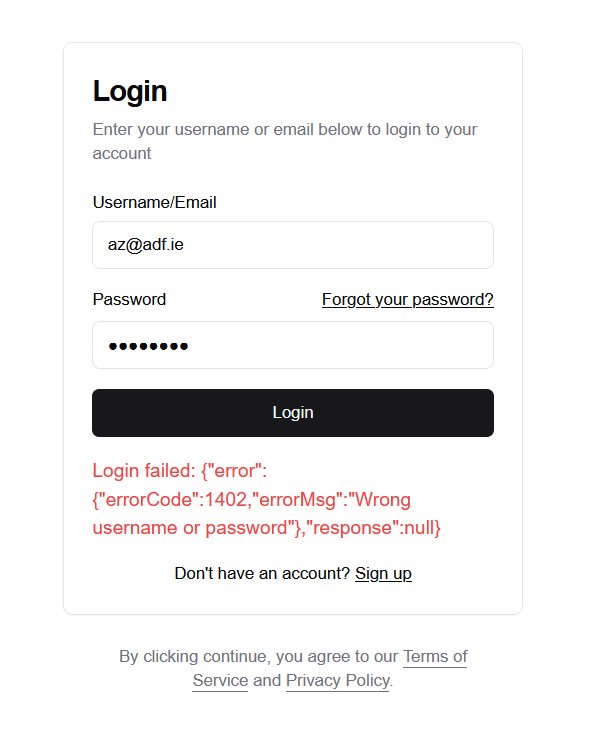
\includegraphics[width=\textwidth]{Figures/fig16.png}}
    \caption{Current error when inputting non-existant username and password}
    \label{fig:plot16}
\end{figure}
\textbf{Overall: }
To resume, Professor Curley found our interface sleek and minimalistic. However, she suggested that if we want to remain with this style, we need to ensure there is as little room as possible for ambiguity and confusion. The user needs to find it easy to move from one feature to another and understand the triggers. Currently, Magpie looks so sleek that the user may not be able to see what they want.\\ \\

\textbf{Survey response}
Below are the answers to the expert review survey in table 3.1. The number next to each multiple choice answer refers to the rating, 1 being the worst and 5 being the best. The response to the survey help complement the oral feedback received during the expert review and provide some quantitative data as a baseline for the next evaluation. The two open-ended questions, to which she asked us to elaborate further, will help us review future open-ended questions and ensure they give enough information for the user to answer.
\begin{table}[h!]
    \centering
    \caption{Expert Review Questionnaire Answers}
    \label{tab:table4}
    \begin{tabularx}{\textwidth}{|p{0.5\textwidth}|X|}
        \hline
        \textbf{Question}                                                                                                        & \textbf{Answer}                                                                                                                                                                                                       \\ \hline
        How user friendly is the log-in/sign up page?                                                                            & Good (4)                                                                                                                                                                                                              \\ \hline
        How user-friendly is the on-boarding process                                                                             & Neutral (3)                                                                                                                                                                                                           \\ \hline
        How effective is the visual hierarchy of the information on the dashboard?                                               & Somewhat effective (4)                                                                                                                                                                                                \\ \hline
        Rate the clarity of the map visualization                                                                                & Average (3)                                                                                                                                                                                                           \\ \hline
        How intuitive is the organization of amenity data categories?                                                            & Neutral (3)                                                                                                                                                                                                           \\ \hline
        Rate the following features from Worst (1) to Best (5)                                                                   & Onboarding: 3, Radius scaling: 4, filter options completeness: 3, profile menu: 1                                                                                                                                     \\ \hline
        How comprehensive is the amenity data coverage for Dublin city?                                                          & Somewhat comprehensive (4)                                                                                                                                                                                            \\ \hline
        How valuable do you think this tool would be for the following use cases - 1: Not valuable at all, 5: Extremely valuable & Urban planning: 4, Resource allocation: 2, Planning permissions: 4, Event planning: 4, Education: 2, Travel planning: 3                                                                                               \\ \hline
        Any additional comments on why this tool would useful/impractical for the above use cases?                               & For each of those user groups, it needs to be signposted more, how they would use them. There is too much left to trying to figure it out yourself. It possibly is very useful for all but needs highlighting by you. \\ \hline
        Evaluate the following technical aspects from Worst (1) to Best (5)                                                      & Loading speed: 3, System responsiveness: 3, Data update frequency: 1, Filter functionality: 3, Radius selection: 4                                                                                                    \\ \hline
        Rate the application's compliance with the items below from Worst (1) to Best (5)                                        & Accessibility: 2, GIS data standards: 3, GDPR: 4                                                                                                                                                                      \\ \hline
        Any additional comments regarding our application?                                                                       & Is loading speed and system responsiveness the same?What does data update frequency mean?                                                                                                                             \\ \hline
    \end{tabularx}
\end{table}

\chapter{Conclusion}
\section{Next steps}
\subsection{Implemented changes}
\begin{itemize}
    \item Fixed authentication bug to ensure user lands on the login page = remedies brusk introduction to Magpie by landing directly on the map
    \item Implementing custom icons with new colors \& larger size  = remedies unclear icons when choosing amenities to display on the map as seen in figure 4.1.
          \begin{figure}
              \centering
              \fbox{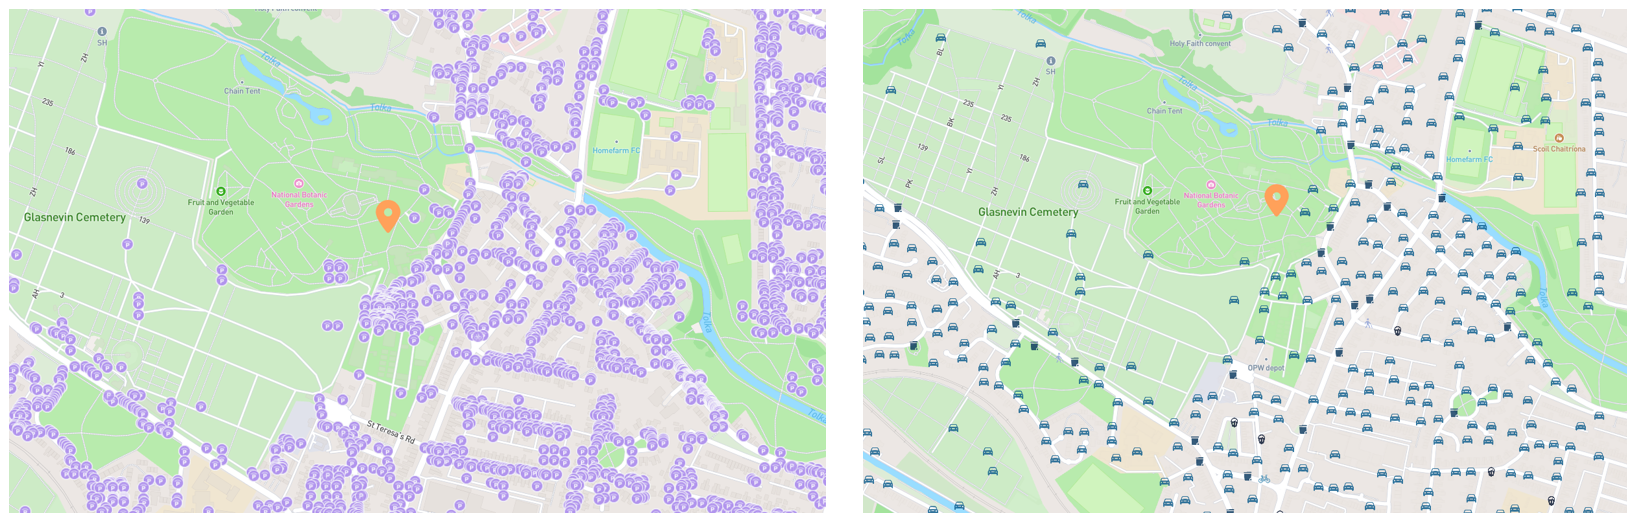
\includegraphics[width=\textwidth]{Figures/fig13.png}}
              \caption{Before and after icon changes}
              \label{fig:plot13}
          \end{figure}
\end{itemize}
\subsection{Planned changes}
\begin{itemize}
    \item Rearrange dashboard to improve workflow and make it easier for the user to navigate the features = remedies confusing workflow of the dashboard
    \item Add amenity icons to the dashboard to help user intuition = remedies disconnect between the map and the dashboard
    \item Add an escape button to the onboarding = remedies locked in the tutorial
    \item Add more features to the radius control to enhance user experience when interacting with it = extra feature
    \item Consolidate certain filter items for easier selection = extra feature
    \item Enhance radius circle format = extra feature
\end{itemize}


% References & Table of Figures Page
\newpage
\addcontentsline{toc}{chapter}{References}
\chapter*{References}
% Use \bibliography{yourbibfile} with a .bib file if available
\begin{itemize}
    \item Lynn, Theodore et al. (Apr. 2023). “Web Accessibility of Irish Local Government Websites”. In: ICDS 2023 : The
          Seventeenth International Conference on Digital Society.
    \item McGuirk, Pauline M and Andrew MacLaran (2001). “Changing approaches to urban planning in an ‘entrepreneurial
          city’: the case of Dublin”. In: European Planning Studies 9.4, pp. 437–457.
    \item Sauro, R. Lewis (April 2009). "Correlations among Prototypical Usability Metrics: Evidence for the Constuct of Usability"
\end{itemize}
\addcontentsline{toc}{chapter}{Table of Figures}
\listoffigures
\listoftables

\end{document}
